\section{Các giải thuật đề xuất giải bài toán tối ưu tuổi thọ mạng cảm biến không dây}
\begin{frame}[noframenumbering]
  \frametitle{Nội dung trình bày}
  \tableofcontents[currentsection]
\end{frame}

\begin{frame}
    \frametitle{Ý tưởng}
    Giải bài toán theo 2 pha:
    \begin{itemize}
        \item Chọn ra các vị trí đặt nút chuyển tiếp.
        \item Tạo kết nối giữa nút cảm biến và nút chuyển tiếp.
    \end{itemize}
\end{frame}

\subsection{Giải thuật di truyền}
\begin{frame}
    \frametitle{Giải thuật di truyền}
    \textbf{Mã hóa cá thể}
    \begin{itemize}
        \item Sử dụng mã hóa nhị phân 
        \item $k = (k_1, k_2,…, k_m)$
        \item[] \begin{equation*}
            k_j = \begin{cases}
                1 & \textrm{nếu có relay triển khai tại $f_j$}\\
                0 & \textrm{nếu ngược lại}
            \end{cases}
        \end{equation*}
    \end{itemize} 
    
    Ví dụ: một cá thể với 10 vị trí khả thi đặt relay

    \begin{figure}[h]
        \centering
        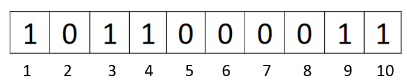
\includegraphics[width=7cm]{picture/indi_encoding.png}
        % \caption{Mã hóa cá thể }
    \end{figure}

    \textbf{Khởi tạo quần thể}

    Tạo ngẫu nhiên các dãy nhị phân độ dài m 
\end{frame}

\begin{frame}
    \frametitle{Giải thuật di truyền}
    
    \textbf{Lai ghép}

    Sử dụng lai ghép một điểm cắt, điểm cắt được chọn ngẫu nhiên
       
    \begin{figure}[h]
        \centering
        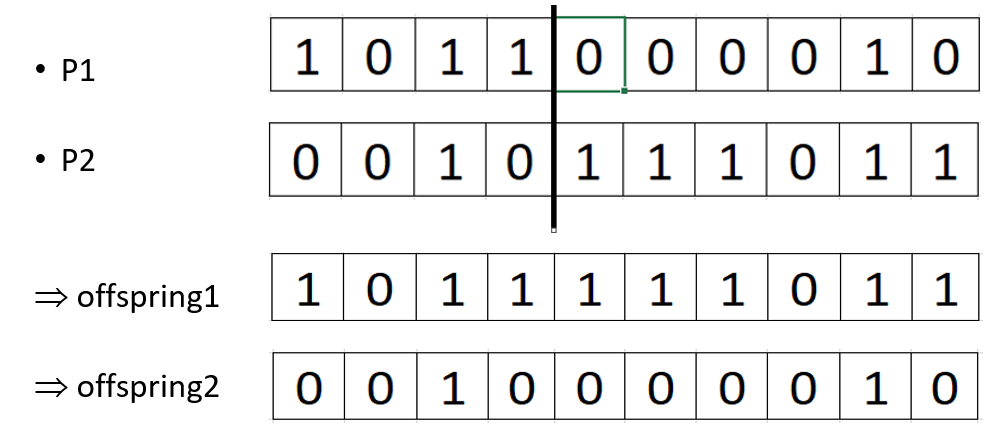
\includegraphics[width=8cm]{picture/crossover.png}
        % \caption{Mã hóa cá thể }
    \end{figure}

\end{frame}

\begin{frame}
    \frametitle{Giải thuật di truyền}
    
    \textbf{Đột biến}
    
    Chọn ngẫu nhiên một bit 0 và một bit 1 trong cá thể, hoán đổi vị trí chúng cho nhau 
       
    \begin{figure}[h]
        \centering
        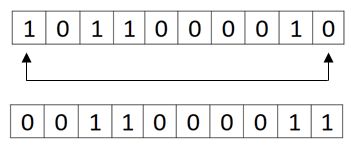
\includegraphics[width=5.5cm]{picture/mutation.png}
        % \caption{Mã hóa cá thể }
    \end{figure}
\end{frame}

\begin{frame}
    \frametitle{Giải thuật di truyền}
    
    \textbf{Tạo kết nối}
    
    Thuật toán heuristic lựa chọn kết nối: với từng nút cảm biến, lựa chọn nút chuyển tiếp sao cho phù hợp
\end{frame}

\begin{frame}
    \fontsize{10pt}{7pt}\selectfont
    \frametitle{Giải thuật di truyền}
       
    \begin{algorithm}[H]
        \SetKwData{Selid}{$sel\_id$}
        \SetKwData{Minmax}{min\_max}
        \SetKwData{Localmax}{local\_max}
        \SetKwData{lossone}{$loss_1$}
        \SetKwData{losstwo}{$loss_2$}
        \SetKwData{Sensors}{S}
        \SetKwData{Relays}{R}
        \SetKwData{Connect}{C}
        \SetKwData{TRUE}{True}
        \SetKwData{FALSE}{False}
        \SetKwData{esensor}{$Et$}
        \SetKwData{erelay}{$Er$}
        \SetKwData{varlthree}{$l_3$}
        \SetKwFunction{MAX}{Max}
        \SetKwFunction{ASSIGN}{Assign}
        \SetKwInOut{Input}{Đầu vào}
        \SetKwInOut{Output}{Đầu ra}
        % \Input{
        %     \\ \Sensors = $\{s_1, s_2, ..., s_n\}$ : tập các sensors 
        %     \\ \Relays = $\{r_1, r_2, ..., r_n\}$: tập các relays 
        %     \\ \Connect: ma trận kết nối 
        %     \\ \esensor, \erelay: năng  lượng tiêu hao của sensors và relays}
        % \Output{\\Các kết nối giữa sensors và relays}
            \SetAlgoLined
            \BlankLine
            \Begin{
                \For{$s_n \in \{s_1, s_2, ..., s_n\}$}{
                    $\Minmax \leftarrow$ INF \\
                    $\Selid \leftarrow 0$ \\
                    \For{$r_n \in \{r_1, r_2, ..., r_n\}$}{
                        $\lossone \leftarrow \esensor_{i, \Selid}$   \\
                        $\losstwo \leftarrow \erelay_j$ \\
                        $\Localmax \leftarrow \MAX(\lossone, \losstwo)$ \\
                        \If {\Minmax < \Localmax} {
                            $\Minmax \leftarrow \Localmax$ \\
                            $\Selid  \leftarrow j$
                        }
                    }
                    $\ASSIGN ~s_i$ to $r_{\Selid}$
                }
            }
            \caption{Connect ($S, R, C, Et, Er$)}      
    \end{algorithm}
\end{frame}

\begin{frame}
    \frametitle{Giải thuật di truyền}
    
    \textbf{Hàm thích nghi}

    Sử dụng hàm mục tiêu của mô hình là hàm thích nghi 

    \vspace{1cm}
    
    \textbf{Chọn lọc}

    \begin{itemize}
        \item Sắp xếp các cá thể theo độ thích nghi, chọn ra các cá thể có độ thích nghi tốt nhất.
        \item Trong trường hợp hai cá thể có độ thích nghi tương đương, sử dụng hàm mục tiêu phụ là tổng năng lượng tiêu hao trong mạng.
    \end{itemize}
   
\end{frame}

\subsection{Phương pháp tìm kiếm cục bộ}
\begin{frame}
    \frametitle{Phương pháp tìm kiếm cục bộ}

    \begin{figure}[h]
        \centering
        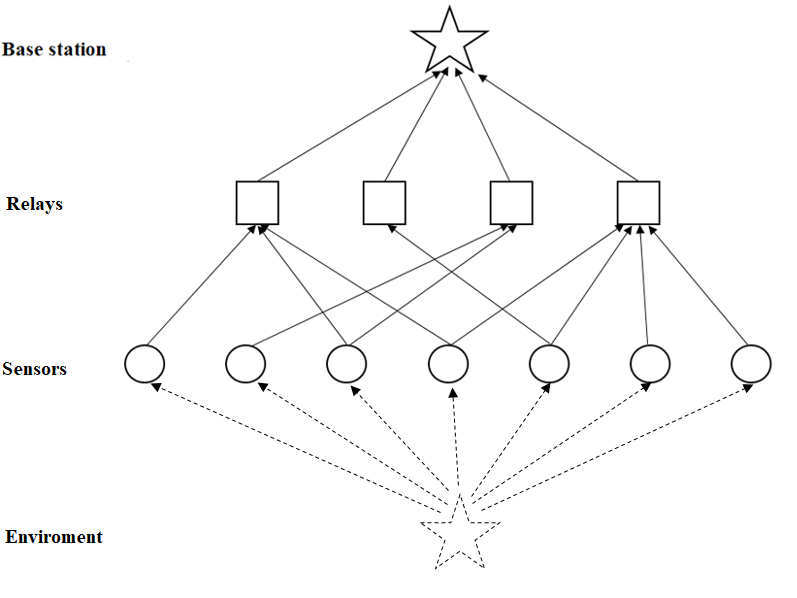
\includegraphics[width=0.9\linewidth]{picture/lite_flow.png}
        % \caption{Mã hóa cá thể }
    \end{figure}
\end{frame}

\begin{frame}
    \frametitle{Phương pháp tìm kiếm cục bộ}

    \textbf{Mã hóa lời giải}
    \begin{itemize}
        \item Vector $k = (k_1, k_2,…, k_m)$.
        \item Trong đó: 
        \begin{itemize}
            \item $k_j$ là số sensor mà relay $j$ kết nối, $1 \leq j \leq m$
            \item $k_j \leq q_j ~\forall 1 \leq j \leq m$ 
            \begin{equation*}
                q_j = \sum_{i = 1}^n c_{ij} ~\forall 1 \leq i \leq n
            \end{equation*}
            \begin{itemize}
                \item[] $q_j$ là số sensor tối đa relay $j$ có thể kết nối
                \item[] $C$ là ma trận kết nối đã nêu trên
            \end{itemize}
            \item Tổng số sensor mà các relay kết nối tới đúng bằng số sensor trong mạng.
            \begin{equation*}
                \sum_{j = 1}^m k_j = n
            \end{equation*}
        \end{itemize}
    \end{itemize}
\end{frame}


\begin{frame}
    \frametitle{Phương pháp tìm kiếm cục bộ}

    \textbf{Toán tử di chuyển}

    \begin{figure}[h!]
        \centering
        \subfigure[Swap]{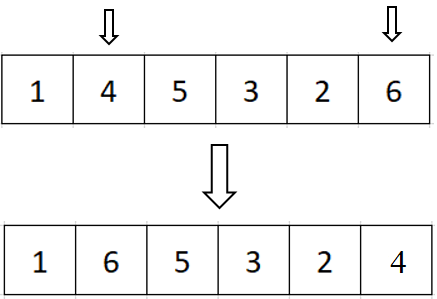
\includegraphics[width=0.35\linewidth]{picture/move1.png}}
        \hspace{1cm}
        \subfigure[Transfer]{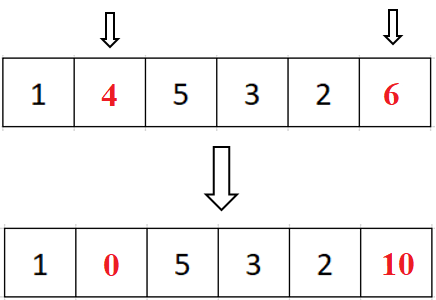
\includegraphics[width=0.35\linewidth]{picture/move2.png}}
        \subfigure[Up-down]{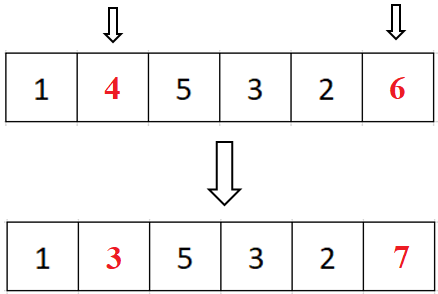
\includegraphics[width=0.35\linewidth]{picture/move3.png}}
    \end{figure}
\end{frame}

\begin{frame}
    \frametitle{Phương pháp tìm kiếm cục bộ}

    \textbf{Lượng giá lời giải}

    \begin{itemize}
        \item Sắp xếp tập các kết nối $E = \{e_1, e_2,…, e_k\}$ trong mạng theo thứ tự không giảm, tập các kết nối đã được sắp xếp $E’ = \{e'_1, e'_2,…, e'_k\}$.
        \item Tìm ra kết nối có chỉ  số nhỏ nhất $e'_i ~(1 \leq i \leq k)$ sao cho với các kết nối $e'_1, e'_2, …, e'_i$ ta giải được bài toán luồng cực đại trong mạng, việc tìm ra kết nối này dựa trên ý tưởng của tìm kiếm nhị phân.
    \end{itemize}
\end{frame}


% Ma gia thuat toan, tam thoi bo 
% \begin{frame}
%     \fontsize{9pt}{10pt}\selectfont
%     \frametitle{Phương pháp tìm kiếm cục bộ}

%     \begin{algorithm}[H]
%         \SetKwData{START}{start}
%         \SetKwData{MID}{mid}
%         \SetKwData{END}{end}
%         \SetKwData{Up}{up}
%         \SetKwData{Energy}{E'}
%         \SetKwData{ivar}{i}
%         \SetKwData{jvar}{j}
%         \SetKwData{TRUE}{True}
%         \SetKwData{FALSE}{False}
%         \SetKwData{varlone}{$l_1$}
%         \SetKwData{varltwo}{$l_2$}
%         \SetKwData{varlthree}{$l_3$}
%         \SetKwFunction{MaxFlow}{MaxFlow}
%         \SetKwFunction{FindConnect}{FindConnect}
%         \SetKwInOut{Input}{Đầu vào}
%         \SetKwInOut{Output}{Đầu ra}
%         % \Input{\\ \Energy : tập các kết nối đã được sắp xếp \\ \ivar và \jvar: chỉ số  bắt đầu và chỉ số kết thúc \\ Năng lượng tiêu hao của các kết nối trong mạng}
%         % \Output{\\Các kết nối được chọn}
%             \SetAlgoLined
%             \BlankLine
%             \Begin{
%                 $\START \leftarrow \ivar$\\
%                 $\END \leftarrow \jvar$\\
%                 $\MID \leftarrow \floor{(\START + \END)/2}$\\
%                 $\varlone \leftarrow \MaxFlow (e'_1, ..., e'_{start})$\\
%                 $\varltwo \leftarrow \MaxFlow (e'_1, ..., e'_{mid})$\\
%                 $\varlthree \leftarrow \MaxFlow (e'_1, ..., e'_{end})$\\
%                 \If{\varlone is \TRUE} {
%                 return $\{e'_1, ..., e'_{start}\}$
%                 }\If{\varlthree is \FALSE} {
%                 return \FALSE
%                 }
%                 \eIf{\varltwo is \FALSE} {
%                     return \FindConnect ($E', mid, end$)
%                 }{
%                     return \FindConnect ($E', start, mid$)
%                 }
%                 \DecMargin{1em}
%             }
%             \caption{FindConnect ($E', i, j$)}      
%     \end{algorithm}
% \end{frame}